\documentclass{article}\usepackage[]{graphicx}\usepackage[]{color}
%% maxwidth is the original width if it is less than linewidth
%% otherwise use linewidth (to make sure the graphics do not exceed the margin)
\makeatletter
\def\maxwidth{ %
  \ifdim\Gin@nat@width>\linewidth
    \linewidth
  \else
    \Gin@nat@width
  \fi
}
\makeatother

\definecolor{fgcolor}{rgb}{0.345, 0.345, 0.345}
\newcommand{\hlnum}[1]{\textcolor[rgb]{0.686,0.059,0.569}{#1}}%
\newcommand{\hlstr}[1]{\textcolor[rgb]{0.192,0.494,0.8}{#1}}%
\newcommand{\hlcom}[1]{\textcolor[rgb]{0.678,0.584,0.686}{\textit{#1}}}%
\newcommand{\hlopt}[1]{\textcolor[rgb]{0,0,0}{#1}}%
\newcommand{\hlstd}[1]{\textcolor[rgb]{0.345,0.345,0.345}{#1}}%
\newcommand{\hlkwa}[1]{\textcolor[rgb]{0.161,0.373,0.58}{\textbf{#1}}}%
\newcommand{\hlkwb}[1]{\textcolor[rgb]{0.69,0.353,0.396}{#1}}%
\newcommand{\hlkwc}[1]{\textcolor[rgb]{0.333,0.667,0.333}{#1}}%
\newcommand{\hlkwd}[1]{\textcolor[rgb]{0.737,0.353,0.396}{\textbf{#1}}}%

\usepackage{framed}
\makeatletter
\newenvironment{kframe}{%
 \def\at@end@of@kframe{}%
 \ifinner\ifhmode%
  \def\at@end@of@kframe{\end{minipage}}%
  \begin{minipage}{\columnwidth}%
 \fi\fi%
 \def\FrameCommand##1{\hskip\@totalleftmargin \hskip-\fboxsep
 \colorbox{shadecolor}{##1}\hskip-\fboxsep
     % There is no \\@totalrightmargin, so:
     \hskip-\linewidth \hskip-\@totalleftmargin \hskip\columnwidth}%
 \MakeFramed {\advance\hsize-\width
   \@totalleftmargin\z@ \linewidth\hsize
   \@setminipage}}%
 {\par\unskip\endMakeFramed%
 \at@end@of@kframe}
\makeatother

\definecolor{shadecolor}{rgb}{.97, .97, .97}
\definecolor{messagecolor}{rgb}{0, 0, 0}
\definecolor{warningcolor}{rgb}{1, 0, 1}
\definecolor{errorcolor}{rgb}{1, 0, 0}
\newenvironment{knitrout}{}{} % an empty environment to be redefined in TeX

\usepackage{alltt}
\usepackage{graphicx, hyperref, soul, float}
\usepackage{amssymb,amsmath,amsthm} 
\usepackage[margin=1.25in]{geometry}


\usepackage[backend=bibtex, natbib=true]{biblatex}
%\addbibresource{../references/references.bib}

\usepackage{color}
\newcommand{\ak}[1]{{\color{magenta} #1}}
\newcommand{\mj}[1]{{\color{blue} #1}}

\theoremstyle{plain}
\newtheorem*{res}{Result}

\title{Bayesian Estimation of the Spectral Density \\ {\small Gaussian IID Case}}
\author{Andee Kaplan \& Maggie Johnson}
\IfFileExists{upquote.sty}{\usepackage{upquote}}{}

\begin{document}

\maketitle

\section*{Purpose}
To check our testing procedure on a model with exact results. This will ensure that our procedure is reasonable and that when we see a periodogram at sparse frequencies does not behave as independent Exponential distribution, that we can trust this result.

\section*{Theoretical Result}

\begin{res}
For $\{X_t\} \stackrel{\text{IID}}{\sim} \text{N}(0,\sigma^2)$, the periodogram values $\left\{ I_n(\omega_j): \omega_j \in \mathcal{F}_n, \omega_j \not\in \{0,\pi\} \right\}$ are IID Exponential($\sigma^2$) random variables.
\end{res}

\section*{Testing Procedure}

\begin{enumerate}
\item Simulate $M$ draws from $X_1,\dots, X_n$ where $\{X_t\} \stackrel{\text{IID}}{\sim} \text{N}(0,\sigma^2)$
\item Obtain $M$ periodograms using the fourier frequencies from $(0, \pi)$, $\omega_j = \frac{2\pi j}{n}: j = 1, \dots, \lfloor n/2 \rfloor$
\item Simulate $M \times n$ draws from $\text{Exp}(\sigma^2)$
\item Multiply periodograms across frequencies to obtain $M$ periodogram products.
\item Multiply exponential draws across $n$ to obtain $M$ draws from the product of exponential distributions (joint distribution)
\item Compare product data using a Kolmogorov-Smirnov test and examining a quantile-quantile plot
\end{enumerate}

We anticipate that the KS test with fail to reject the null hypethesis, giving no indication that the samples are drawn from different distributions. Similarly, we expect that the quantile-quantile plot comparing the periodogram to exponentials should indicate a good fit.

\section*{Results}
Using $M = 1000, n = 500, \sigma^2 = 1$, the K-S test statistic and p-value are:
\begin{knitrout}
\definecolor{shadecolor}{rgb}{0.969, 0.969, 0.969}\color{fgcolor}\begin{kframe}
\begin{verbatim}
## 
## 	Two-sample Kolmogorov-Smirnov test
## 
## data:  perio.prod and exp.prod
## D = 0.03, p-value = 0.7591
## alternative hypothesis: two-sided
\end{verbatim}
\end{kframe}
\end{knitrout}

From these results we fail to reject $\text{H}_0$, which states that the two samples are from the same distribution. Thus there is no evidence that our periodogram values at the fourier frequencies are not independent Exponential($\sigma^2$) random variables. This is consistent with our expectations. Let us also take a look at the quantile-quantile plot.
\begin{knitrout}
\definecolor{shadecolor}{rgb}{0.969, 0.969, 0.969}\color{fgcolor}\begin{figure}[H]


{\centering 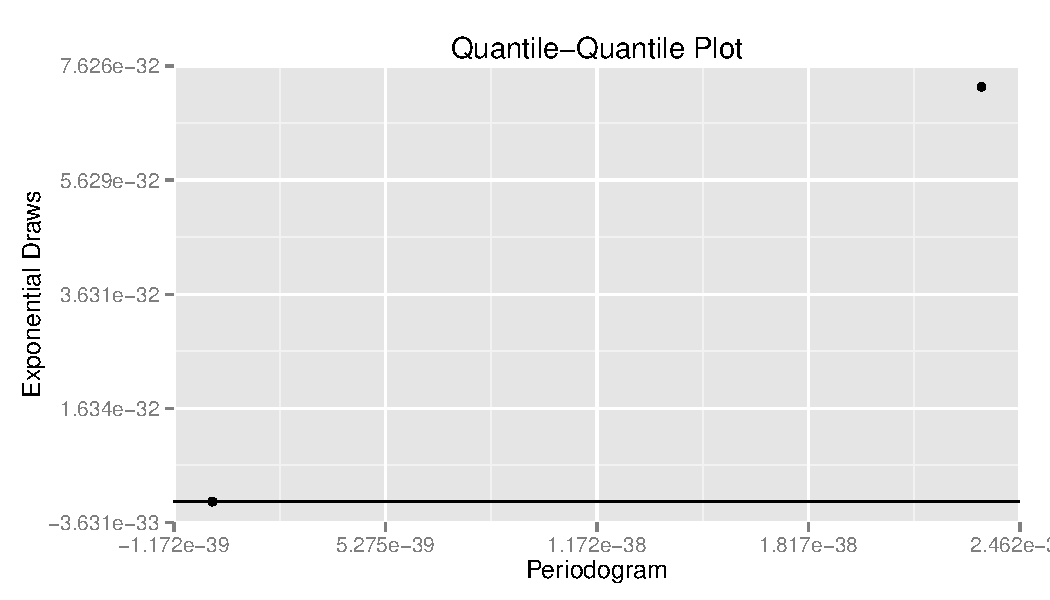
\includegraphics[width=0.8\textwidth]{figure/qqplot} 

}

\caption[Quantile-quantile plot of the product of periodogram values at the Fourier frequencies versus the product of Exp(1) draws]{Quantile-quantile plot of the product of periodogram values at the Fourier frequencies versus the product of Exp(1) draws.\label{fig:qqplot}}
\end{figure}


\end{knitrout}

Clearly, this does not show a good fit between our exponential draws and the periodograms of simulated IID Gaussian data. All of our samples are actually very close to zero.
% latex table generated in R 3.0.2 by xtable 1.7-1 package
% Wed Dec 04 22:05:11 2013
\begin{table}[H]
\centering
\begin{tabular}{rrrrrrr}
  \hline
 & Min. & 1st Qu. & Median & Mean & 3rd Qu. & Max. \\ 
  \hline
Periodogram & 1.5500E-95 & 5.7500E-69 & 4.0800E-63 & 2.9300E-41 & 2.5800E-57 & 2.3400E-38 \\ 
  Exponential & 2.3300E-93 & 2.2000E-69 & 3.9900E-63 & 7.3100E-35 & 3.3100E-57 & 7.2600E-32 \\ 
   \hline
\end{tabular}
\caption{Summaries of the products across frequencies of sample periodograms and samples from the Exponential($\sigma^2$) distribution.} 
\end{table}


To further investigate the relationship, we look at the quantile-quantile plot for only the first half of quantiles.
\begin{knitrout}
\definecolor{shadecolor}{rgb}{0.969, 0.969, 0.969}\color{fgcolor}\begin{figure}[H]


{\centering 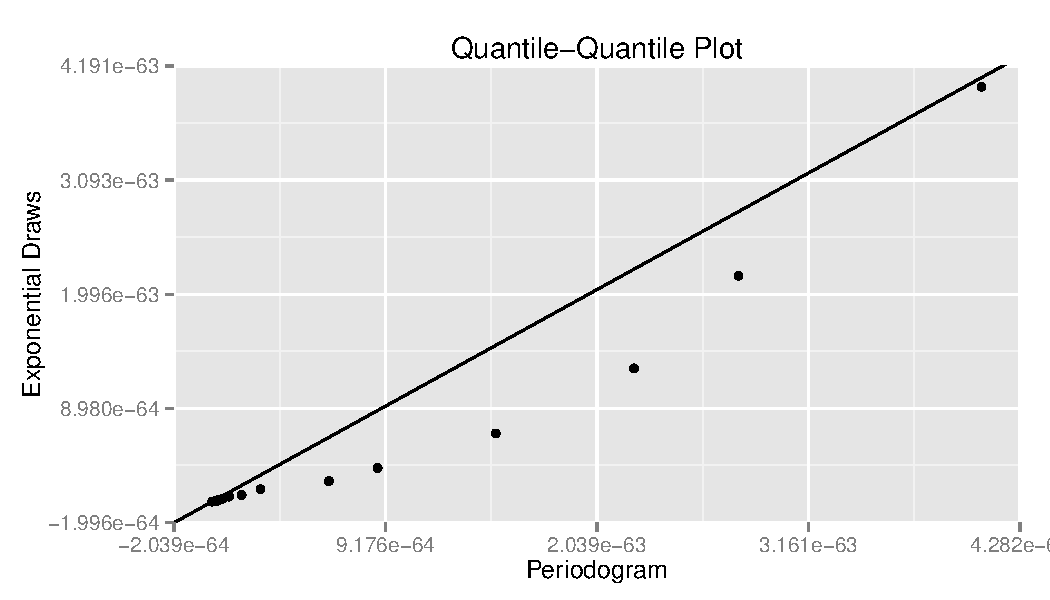
\includegraphics[width=0.8\textwidth]{figure/qqplot2} 

}

\caption[Quantile-quantile plot of the product of periodogram values at the Fourier frequencies versus the product of Exp(1) draws]{Quantile-quantile plot of the product of periodogram values at the Fourier frequencies versus the product of Exp(1) draws.\label{fig:qqplot2}}
\end{figure}


\end{knitrout}

By zooming in on the first half of the points we can see there is a closer relationship between the quantiles, however not as linear as we would expect, given the exact result above. 

\section*{The Problem}
By taking the product of our periodograms (and exponential draws) over each frequency $\frac{n}{2}$ times, we are essentially amplifying the probability of obtaining values very close to zero. To illustrate this behavior, compare the Exp(1) density to the product of 50 Exp(1) densities.
\begin{knitrout}
\definecolor{shadecolor}{rgb}{0.969, 0.969, 0.969}\color{fgcolor}\begin{figure}[H]

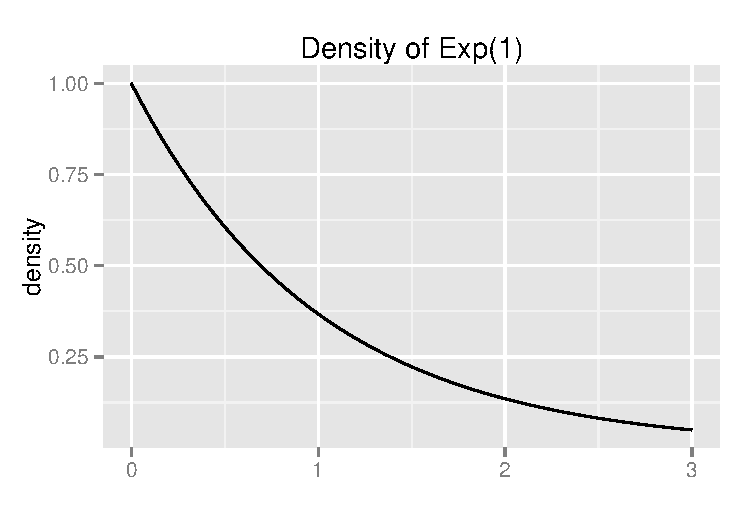
\includegraphics[width=.49\textwidth]{figure/density1} 
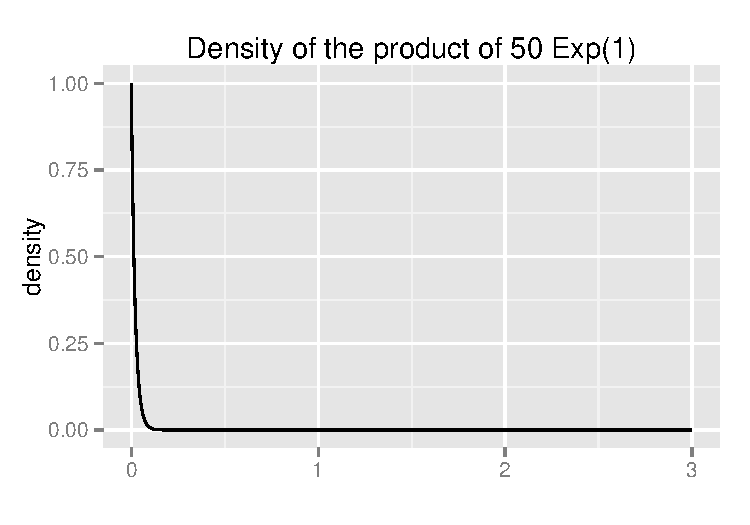
\includegraphics[width=.49\textwidth]{figure/density2} \caption[Comparison of the Exp(1) density to the product of 50 Exp(1) densities]{Comparison of the Exp(1) density to the product of 50 Exp(1) densities.\label{fig:density}}
\end{figure}


\end{knitrout}

In our example above, we are actually taking the product of 249 Exp(1) distributions, leading to many values almose indistinguishable from zero (in the order of $10^-95$).

With this in mind, the question becomes {\bf how robust is the Kolmogorov-Smirnov test to many values close to zero and is there a better way to test for independence as well as distribution?}

\end{document}
